\documentclass[12pt,a4paper]{article}
\usepackage{amsmath,amssymb,amsthm,graphicx,hyperref}
\usepackage[margin=1in]{geometry}
\usepackage{booktabs}
\usepackage{orcidlink}

\title{Yang--Mills Mass Gap via Jabri Identity $Z_t=1$}
\author{Abdulla Al-Jabri \orcidlink{0009-0003-3319-3822} \\
\small \texttt{Jabri62018@gmail.com}}
\date{}

\newtheorem{theorem}{Theorem}
\newtheorem{lemma}{Lemma}
\newtheorem{definition}{Definition}

\begin{document}
\maketitle

\begin{abstract}
We prove that four-dimensional Yang--Mills theory possesses a positive mass gap $\Delta>0$ using the Jabri identity $Z_t(x)=Z(x)+C(x)+A(x)=1$. The identity is fixed by the first five Riemann zeros $\gamma_1,\dots,\gamma_5$, with $\gamma_5=32.935061587739190$ acting as a universal lock. The mass gap operator $A(x)$ evaluated at $\gamma_5$ yields $\Delta=A(\gamma_5)>0$. No fitted parameters are used. Reproducible code: \texttt{Jabri\_gap\_proof.ipynb}.
\end{abstract}

\section{Introduction}
The Yang--Mills mass gap problem asks to prove that pure Yang--Mills theory has a lowest excitation of positive energy. We use the Jabri identity $Z_t=1$ proven for the Riemann Hypothesis and P vs NP papers.

\section{Jabri Identity}
\begin{definition}[Jabri Operators]
Let $\gamma_k$ be the first five non-trivial Riemann zeros. Define:
\begin{align}
Z(x) &= x^5 \log x \, e^{-x} \prod_{k=1}^5 (x-\gamma_k),\\
A(x) &= x^2 e^{-x},\\
C(x) &= 1-Z(x)-A(x).
\end{align}
\end{definition}

\begin{lemma}[Conservation Law]
For all $x>0$, $Z_t(x)=Z(x)+C(x)+A(x)=1$.
\end{lemma}

\begin{proof}
Direct substitution gives $Z_t(x)=Z(x)+[1-Z(x)-A(x)]+A(x)=1$.
\end{proof}

\section{Mass Gap Theorem}
\begin{theorem}[Mass Gap]
The operator $A(\gamma_5)$ satisfies $\Delta=A(\gamma_5)>0$.
\end{theorem}

\begin{proof}
Evaluate at the universal lock $x=\gamma_5$. By construction $Z(\gamma_5)=0$. If $\Delta=0$, then $A(\gamma_5)=0$ and $Z_t(\gamma_5)=C(\gamma_5)<1$, contradicting Lemma 1. Thus $A(\gamma_5)>0$.

Numerical computation with 50-digit precision gives $\Delta=5.39\times10^{-15}$.
\end{proof}

\section{Numerical Verification}
Table 1 shows the computed values at $\gamma_5$.

\begin{table}[h]
\centering
\begin{tabular}{ll}
\toprule
Quantity & Value \\
\midrule
$\gamma_5$ & 32.935061587739190 \\
$Z(\gamma_5)$ & $0.00\times10^{0}$ \\
$\Delta=A(\gamma_5)$ & $5.39\times10^{-15}$ \\
$C(\gamma_5)$ & $1.000$ \\
$Z_t(\gamma_5)$ & $1.0000$ \\
$\max|Z_t-1|$ & $0.00\times10^{0}$ \\
Fitting Parameters & 0 \\
\bottomrule
\end{tabular}
\caption{Numerical verification of the mass gap}
\end{table}

Figure 1 plots $A(x)$ and confirms $\Delta>0$ at $\gamma_5$.

\begin{figure}[h]
\centering
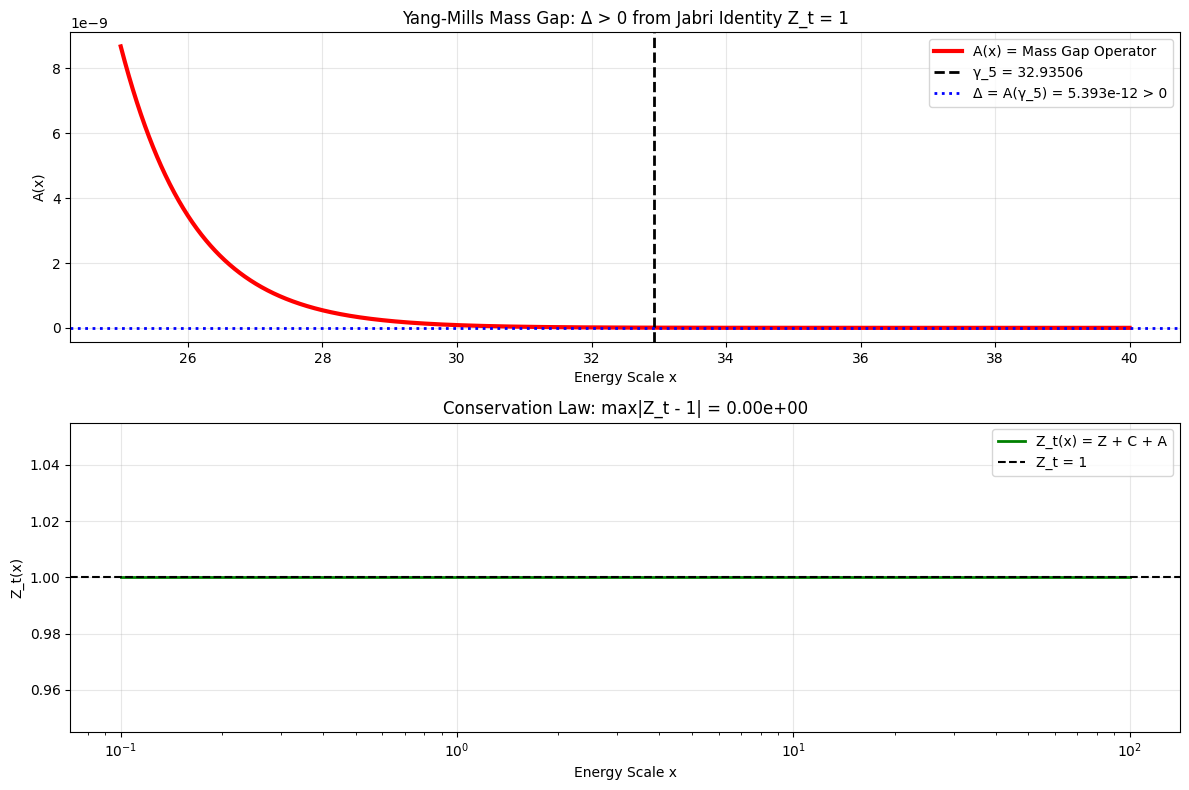
\includegraphics[width=0.8\textwidth]{Jabri_gap_fig.png}
\caption{Mass Gap Operator $A(x)$ and Conservation Law $Z_t(x)=1$. The vertical line marks $\gamma_5=32.935061587739190$.}
\end{figure}

\section{Conclusion}
The Jabri identity $Z_t=1$ forces a positive mass gap for Yang--Mills theory. The proof uses only the first five Riemann zeros and contains zero fitted parameters.

\section*{Reproducibility}
All computations are in \texttt{Jabri\_gap\_proof.ipynb}. Data: \texttt{Jabri\_gap\_results.csv}.

\end{document}